\chapter{Przykład użycia}
\label{sec:useexample}
10 %
Poniższy rozdział zawiera przykład użycia stworzonej aplikacji. Prezentuje jedynie niewielką część możliwości.


\section{Historia USA}
\label{sec:usahistory}

W celu zobrazowania powstawania USA poniżej zaprezentowano 3 stany jego rozwoju. Na rysunku \ref{fig:st1} znajduje się obszar państwa w momencie ratyfikacji konstytucji.Kolorem czarnym zaznaczone są 13 pierwszych stanów które uznawane są za założycielskie. Pokazano również możliwość dodawania opisu do wydażeń dodanych do sceny, umożliwia to dodanie dodatkowych informacji które mogą wspomóc proces dydatktyczny.

\begin{figure}[H]
  \centering
    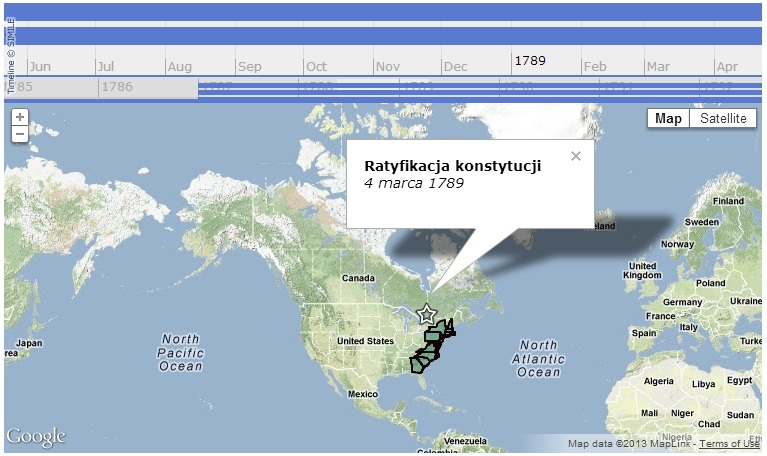
\includegraphics[width=100mm]{ge/st1.jpg}
  \caption{rok.}
  \label{fig:st1}
\end{figure}

Kolejny rysunek \ref{fig:st2} opisuje stan z 1912 roku. Dzięki możliwości stworzenia dwuch lub pasm które będą odpowiadały za zmianę daty, przesunięcie się o ponad 100 lat nie sprawia większego trudu i możliwe w krótkim czasie.

\begin{figure}[H]
  \centering
    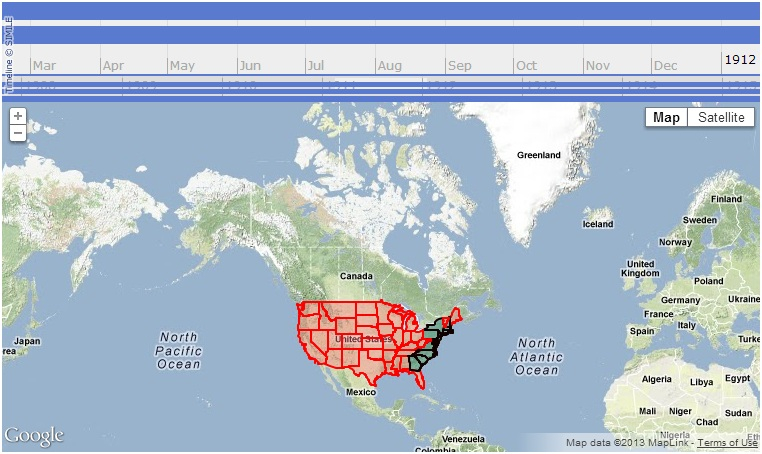
\includegraphics[width=100mm]{ge/st2.jpg}
  \caption{rok.}
  \label{fig:st2}
\end{figure}

Ostani element tej serii ukazuje aktualny stan granic. Widać że utrzymuje się on od 1959 roku.

\begin{figure}[H]
  \centering
    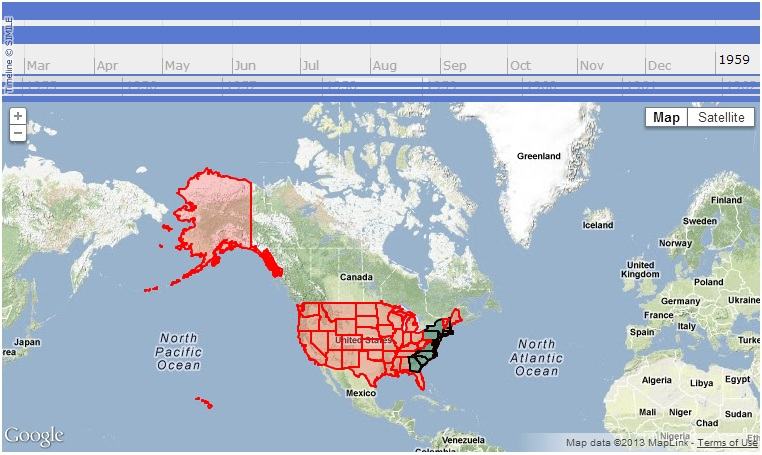
\includegraphics[width=100mm]{ge/st3.jpg}
  \caption{rok.}
  \label{fig:st3}
\end{figure}
